\section{Control Method} \label{sec:control_method}

In this section we combine sampling, barrier functions and energy tank into a model-based method for robust and safe interaction control. First the sampling method is presented with a brief explanation of each cost components. Afterwards, the CBFs are formulated for the manipulation task. Ultimately, a passivity analysis of the system allows the integration of an energy tank to ensure autonomous passivity. 

\subsection{Sampling-based control}
The sampling-based framework offers the freedom to directly plan in torque space or use position/velocity control and defer tracking to a low-level controller. In fact, directly planning in the joint space allows to account for objectives which are not in the operational control space such as joint limits and self-collision avoidance. The internal model used to sample trajectory rollouts has the same form as in \eqn \ref{eq:eom}. Joint velocity commands are sampled and then translated to motor torques:
\begin{equation}
    \vect{\tau}_{ctrl} = \matr{K}_{p} (\command - \dconfigRobot) + \robotCoriolis,
\end{equation}
with an appropriate choice of the positive-definite diagonal gain matrix $\matr{K}_{p} \in \nR{\robotDoF\times\robotDoF}$. 

\subsection{Cost shaping}
As described in Section~\ref{sec:formulation}, the control objective is to drive the system to a desired state. Furthermore, as state constraints are not explicitly taken into account by the formulation, a common heuristic is to penalize deviations from feasible states in the cost function. Input constraints are easier to handle as the non-linear dynamics can be augmented with a function that projects the sampled inputs to the feasible set $\mathcal{U}$. In the following we define several cost components associated with the different high-level objectives and constraints.
We denote by $\mathds{1}[\cdot]$ the \textit{indicator function} such that
\begin{equation}
    \mathds{1}[x] = 
    \begin{cases}
    1 & \text{if } x \text{ is True} \\
    0 & \text{otherwise}
    \end{cases}.
\end{equation}
In the following we drop from the notation the dependence from the current state. 

\paragraph{Target reaching} in the target reaching task, the goal is to bring a frame attached to the robot (generally the end-effector frame) to a desired pose. We define with the vector $\vect{p}$ the current frame pose and $\vect{p}^*$ the desired target. The \textit{tracking cost} is computed as a weighted distance between these quantities. The distance is computed in the tangent space to $SE(3)$ using the logarithmic mapping~\cite{blanco2010tutorial}:
\begin{equation} \label{eq:tracking_cost}
     c_{t} = || \log(\vect{p} - \vect{p^{*}}) ||^2_{\weightMatrix{t}},
 \end{equation}
 where $\weightMatrix{t}$ is a diagonal weight matrix used to penalize the translation and rotation errors. Also note that the current end-effector pose $\vect{p}$ is a function of the robot configuration $\configRobot$, computed by evaluating the forward kinematics.
 
 \paragraph{Collision avoidance} let $\contact \in \{0, 1\}$ represent an auxiliary variable which is equal to 1 when the manipulator is in contact with the environment. The value of $\contact$ can be computed by evaluating the forward kinematics for the current configuration and searching for collisions between bodies. 
 $\contact$ is used to avoid collisions during contact-free motions of the end-effector. 
 %Although not developed in the presented solution, one could differentiate contacts between each body pair and also penalize self-collision. 
 The \textit{contact cost} is defined as
 \begin{equation}
     c_{\contact}= \weightScalar{\contact} \contact(\state), 
 \end{equation}
where $\weightScalar{\contact} \in \nR{}_{\geq 0}$. 
 A similar technique can be used to consider contacts between joints and penalize self-collisions. 

 \paragraph{Joint position limits} the manipulator is subject to physical joint limits and velocity limits. The first can be addressed by introducing a cost component that penalizes violation of the constraints. We define the \textit{joint limits cost} with:
 \begin{align}
     &c_{j} = \mathds{1}[\configRobot > \upperLimits](\weightScalar{j} + ||\upperLimits - \configRobot)||^2_{\weightMatrix{js}}) + \nonumber\\ 
     &\qquad\mathds{1}[\configRobot < \lowerLimits](\weightScalar{j} +  || \configRobot - \lowerLimits||^2_{\weightMatrix{js}}), 
 \end{align}
 where the scalar $\weightScalar{j}$ is a constant cost added when the limit is violated. The matrix $\weightMatrix{js}$ adds a quadratic term in the limit violation. This was shown in~\cite{williams_information-theoretic_2018} to help the controller find its way back if poor sampling brings the system outside of the joint position limits.
 
 \paragraph{Arm reach} we introduce an additional term that penalizes configurations where the arm's end-effector moves far from the base. This helps to select solutions where base motion is preferred over stretching the arm which can lead to singular configurations. The translation vector from the end-effector frame $E$ to the arm base frame $B$ is defined with the vector $\vect{t}_{BE}$. The current reach is then $r_{\text{curr}} = || \vect{t}_{BE} ||_2$. Given a maximum reach $r_{\text{max}} \in \nR{}_{\geq 0}$, the \textit{reach cost} is then defined by:
 \begin{equation}
   c_r = \mathds{1}[r_{\text{curr}} > r_{\text{max}}] (\weightScalar{r} + \weightScalar{rs}(r_{\text{curr}} - r_{\text{max}})^2),    
 \end{equation}
 with an appropriate choice of positive scalar weights $\weightScalar{r}$ and $\weightScalar{rs}$ as a constant term and a quadratic term in the violation.
 
 \paragraph{Self collision avoidance} similarly to the arm reach, the self collision avoidance can be implemented as an additional cost term which is active when the distance between a pair of frame is less then a pair-dependent threshold. Given the distance between two frames $d_{ij}$ and a threshold $d^{min}_{ij}$ the self collision cost for the pair reads:
 \begin{equation}
   c_{sc} = \mathds{1}[d_{ij} < d^{min}_{ij}] (\weightScalar{r} + \weightScalar{rs}(d^{min}_{ij} - d_{ij})^2),    
 \end{equation}
 
 \paragraph{Object manipulation} in the manipulation task the goal is to change the state of an articulated object through interaction. The \textit{manipulation cost} penalizes deviations from the target object configuration $\configObject^{*}$,
\begin{equation}
    c_o(\configObject; \weightMatrix{o}) = || \configObject - \configObject^{*}||^2_{\weightMatrix{o}}.
\end{equation}
\paragraph{Power minimization} we propose a new cost component that taking into account the power dissipated to perform the task, can help to regulate the interaction wrench. We leverage the fact that as rollouts are performed in simulation, the joint torque generated through interaction can be easily computed summing the contribution of each force $F_c$ at each contact point $c$:
\begin{equation}
\boldsymbol{\tau}_{ext} = \sum\limits_{c} \matr{J}_c F_c    
\end{equation}
where $\matr{J}_c$ is the contact jacobian. The power dissipated during the task is therefore $-\boldsymbol{\tau}_{ext}^T\command$ which is positive when acting "against" the environment. Cost associated to power penalization is:
\begin{equation}
   c_p = \max(0, -\weightScalar{p} \boldsymbol{\tau}_{ext}^T\command - p_{max})      
 \end{equation}
where $p_{max}$ is the maximum power that can be dissipated during the task.
As we will later see, this is the power that is drained from the tank and therefore, this cost component has the additional benefit to help avoiding drainage of the energy tank.
 
\subsection{Cost scheduling}
The manipulation task consists of two phases. In a first phase the manipulator reaches the proximity of the object to be manipulated while avoiding hard collisions with the object. This step brings the robot end-effector close to an estimated contact point, allowing for a fast and successful exploration in the following manipulation phase. In the second phase, the goal is to bring the object to the desired state while keeping the end-effector close to the initial guess. This switch is enabled turning on the object manipulation cost $c_o$. The stage costs inform the controller about the different objectives in each of the described steps:
We decide to keep separate target reaching weight matrices $\weightMatrix{t}^{r}$ and $\weightMatrix{t}^{m}$ as this offers more flexibility in the cost design. As we will show in Section~\ref{sec:experiments}, a reducing the end effector positioning penalty during the manipulation phase allows the controller to choose trajectory that fully exploit the contact dynamics. This approach is in contrast with previous works where manipulation generally follows a prescribed grasping state~\cite{abraham_model-based_2020}. Grasping introduces a kinematic constraint that, while reducing the optimal control search space, does not allow for more flexible, contact-based behaviors to emerge such as pulling, pushing or sliding. 

\subsection{Barrier Functions}
In the previous paragraph a combination of cost components where introduced in order to address both performance and safety. The variety of objectives makes the cost landscape highly complex which can be detrimental for trading-off performance against safety requirements. In the following, we look at how barrier functions can encode safety-critical constraints. We start deriving the CBF constraints based on differential kinematics equation
\begin{equation}
    \dot{\state} = \matr{J} \dconfigRobot
\end{equation}
As described in \cite{benzi2021optimization}, a simple CBF can be derived for each joint to keep it between its lower and upper bounds $q_i^-$ and $q_i^+$ respectively:
\begin{equation}
h_{ql}^i = \epsilon_{ql} \frac{(q_i^+ - q)(q - q_i^-)}{(q_i^+ - q_i^-)}
\end{equation}
In the following we treat the safety requirements associated to robot frames and denote with $\vect{x}^p_{i} \in \nR{3}$ the position of frame $i$ computed through forward kinematics.  
The self collision safe set can be obtained approximating potentially colliding frames with non intersecting spheres. Then the self-collision CBF is defined as
\begin{equation}
    h_{sc}^{ij} = \frac{1}{2}(||\vect{x}^p_i - \vect{x}^p_j||^2 - D_c^2)
\end{equation}
associated with the collision pair composed by the $i$th  and $j$th robot frames. Note that we can similarly formulate a constraint encoding arm reach limits. In fact, the following is a valid zeroing CBF, positive only when the end effector is within the prescribed reach with respect to the arm base,
\begin{equation}
    h_{ar} = \frac{1}{2}(D_r^2 - (\vect{x}^p_{ee} - \vect{x}^p_{base})^T P (\vect{x}_{ee} - \vect{x}_{base}) )
\end{equation}
The projection matrix $P = \text{diag}(1, 1, 0) \in \nR{3 \times 3}$ makes sure that the reach is only computed in the 2d plane. Each of this CBF translates to a constraint of the form in \eqn \ref{eq:cbf-const} which is affine in the joints velocity command. 

\subsection{Energy Tank}
As described in \sect \ref{sec:theory}, energy tanks can be used to \emph{passify} the system, hence to ensure stability. Inspired by the work in \cite{benzi2021optimization} and \cite{shahriari2018valve}, this adaptation naturally fits the control method so far developed. The system model is first augmented with a virtual tank. As a consequence, the forward simulation of each rollout also contains the time evolution of the tank energy and this can be used to ensure passivity in a \emph{predictive} manner. We are left with the task of defining which are the \emph{power ports} connected to the tanks such that passivity is preserved. To this end, we perform a passivity analysis of the \emph{real} system. Its 
velocity controller obeys to a dynamically compensate PI control law:
\begin{equation}
\commandTorque = \coriolis \dconfigRobotDesired + g(\configRobot) - \matr{K}_D \dconfigRobotError - \matr{K}_I \int\limits_{0}^{\sigma} \dconfigRobotError\ dt
\end{equation}
 with the auxiliary error variables
\begin{align*}
    \configRobotError &=  \configRobot - \configRobotDesired \\
    \dconfigRobotError &=  \dconfigRobot - \dconfigRobotDesired \\
    \ddconfigRobotError &=  \ddconfigRobot - \ddconfigRobotDesired |_{\ddconfigRobotDesired = 0} = \ddconfigRobot
\end{align*}
We define the system energy as 
\begin{equation}
    S_{robot} = \frac{1}{2} \dconfigRobotError^T \massMatrix \dconfigRobotError + \frac{1}{2} \configRobotError^T \matr{K}_P \configRobotError
\end{equation}
The energy dynamics can be obtained computing the time derivative of the previous expression. Plugging in \eqn \eqref{app:dynamics} and exploiting the fact that $\massMatrix - 2 \coriolis$ is skew symmetric we get:
\begin{equation}
\begin{aligned}
    \dot{S}_{robot} &= \dconfigRobotError^T \massMatrix \ddconfigRobotError + \frac{1}{2} \dconfigRobotError^T \dot{\massMatrix} \dconfigRobotError + \dconfigRobotError^T \matr{K}_P \configRobotError \\
    &= \dconfigRobotError^T \left[ -\coriolis \dconfigRobotError - \matr{K}_P \configRobotError - \matr{K}_D \dconfigRobotError - \matr{K}_I \int\limits_{0}^{\sigma} \dconfigRobotError + \externalTorque \right] \\
    &+ \frac{1}{2} \dconfigRobotError^T \dot{\massMatrix} \dconfigRobotError + \dconfigRobotError^T \matr{K}_P \configRobotError \\
    &= -\dconfigRobotError^T \matr{K}_P \configRobotError + \dconfigRobotError^T \externalTorque + \frac{1}{2} \dconfigRobotError^T \underbrace{\left[ \dot{\massMatrix} - 2\coriolis \right]}_{=0} \dconfigRobotError \\
    &- \dconfigRobotError^T \matr{K}_D \dconfigRobotError  - \dconfigRobotError^T \matr{K}_I \int\limits^{\sigma}_{0} \dconfigRobotError\ dt\\
    &= \dconfigRobotError^T \matr{K}_P \dconfigRobotError + \dconfigRobotError^T \externalTorque - \dconfigRobotError^T \matr{K}_D \dconfigRobotError -  \dconfigRobotError^T \matr{K}_I \int\limits^{\sigma}_{0} \dconfigRobotError\ dt  
\end{aligned}
\end{equation}
As we compute the desired position integrating the desired velocity over time, it holds that 
\begin{equation}
    \configRobotError = \int\limits^{\sigma}_{0}
    \dconfigRobotError\ dt
\end{equation}
We choose $K_P = K_I$ obtaining
\begin{equation}
    \dot{S}_{robot} = \dconfigRobotError^T \externalTorque - \dconfigRobotError^T \matr{K}_D \dconfigRobotError \leq \dconfigRobotError^T \externalTorque 
\end{equation}
It is clear that while the dissipative term passifies the system, the external torque can lead to a loss of passivity. Since the environment is passive, it exists an environment energy such that ~\cite{shahriari2018valve}
\begin{equation}
    \dot{S}_{env} \leq -\dconfigRobot^T \externalTorque
\end{equation}
The energy tank is finally connected to the system through the power port $(\dconfigRobot^*, \externalTorque)$ and therefore
\begin{equation} \label{eq:tank_dynamics}
\dot{S}_{tank} = \dconfigRobot^{*T} \externalTorque 
\end{equation}
The time evolution of the autonomous system's energy is
\begin{equation}
\begin{aligned}
    \dot{S}_{tot} &= \dot{S}_{robot} + \dot{S}_{tank} + \dot{S}_{env} \\
    &\leq \dconfigRobotError^T \externalTorque + \dconfigRobot^{*T} \externalTorque - \dconfigRobot^T \externalTorque \leq 0
\end{aligned}
\end{equation}
showing the system passivity. The increase of the robot energy is compensated by a reduction of the tank energy. The new optimization problem has the form as in \eqn \ref{eq:cbf-qp} but with the additional passivity constraint 
\begin{equation}
    \int\limits_{0}^{\sigma} \boldsymbol{\tau}_{ext}^T \command \ dt \geq -S(x_t(0)) + \epsilon + \delta_t
\end{equation}
with $\delta_t$ the slack variable associated with the passivity constraint. 
\add{figure showing the interconnection between all the blocks}


\subsection{Closing the loop}
As described in \sect \ref{sec:theory}, we can formulate a quadratic program to find the input velocity which is the closest to the sampled policy while also satisfying the constraints.
\begin{mini}|s| 
{\tilde{\vect{u}}_t, \boldsymbol{\delta}}{||\tilde{\vect{u}}_t - \command_t||^2 + \boldsymbol{\delta}^T \matr{P} \boldsymbol{\delta}\quad \text{(FILTER-QP)}}{}{\label{eq:cbf-qp}}
\addConstraint{\dot{h}^i_{ql} \geq -{h}_{ql} + \delta^i_{ql} \quad \forall \ i \in [1,  m] }{}{\quad \text{(Joint Limits)}}
\addConstraint{\dot{h}^{ij}_{sc} \geq -{h}_{ij} + \delta^{ij}_{sc} \quad \forall \ (i,j) \in \mathcal{I}}{}{\quad \text{(Self Collision)}}
\addConstraint{\dot{h}^i_{ar} \geq -{h}_{ar} + \delta^i_{ar}}{}{\quad \text{(Arm Reach)}}
\addConstraint{\int\limits_{0}^{\sigma} \boldsymbol{\tau}_{ext}^T \command \ dt \geq -S(x_t(0)) + \epsilon + \delta_t}{}{\quad \text{(Passivity)}}
\addConstraint{\tilde{\vect{u}}_t \in \mathcal{U}}{}{\quad \text{(Input Limits)}}
\end{mini}
where $\boldsymbol{\delta}$ is the vector of slack variables and $\matr{P}$ is a positive definite diagonal matrix. Finally, the set denoted by $\mathcal{I}$ is the set of collision link pairs.  We name this problem FILTER-QP as it changes the control input only it is unsafe or causes a loss of passivity. Instead of simply applying this optimization point-wise, we \emph{filter} the full input sequence in a sequential manner. At every time step, a QP is solved providing a new input which is used to advance the system to the next time step as shown in \algo \ref{algo:sequential_qp}. The new filtered input trajectory is then used as new policy parametrization, to warm start a new round of rollouts sampling. 

\begin{algorithm}
\caption{Sequential FILTER-QP \label{algo:sequential_qp}}
\KwData{optimal input sequence $U_t = [\command_t, \command_{t+1}, \dots, \command_{t+T-1}]$, current state $\vect{x}_t$, 
tank state $x_t$}
\KwResult{filtered input trajectory $\bar{U}_t$}
$\vect{x} \gets \vect{x}_t$\;
$\command \gets \command_t$\;
$n \gets 0$\;
\While{$n < T$}{
  $\bar{\command}_{t+n} \gets \text{FILTER-QP}(\vect{x}, \command, x_t, \boldsymbol{\tau}_{ext})$ \hfill (\eqn \ref{eq:cbf-qp}) \\
  $\vect{x}, \boldsymbol{\tau}_{ext} \gets $Step Simulation \hfill (\eqn \ref{eq:eom})\\
  $x_t \gets$ Integrate Tank \hfill (\eqn \ref{eq:tank_dynamics}) \\
  $\command \gets \bar{\command}_{t+n}$ \\
  $n = n + 1$
}
\end{algorithm}

\begin{figure}[h!]
\centering
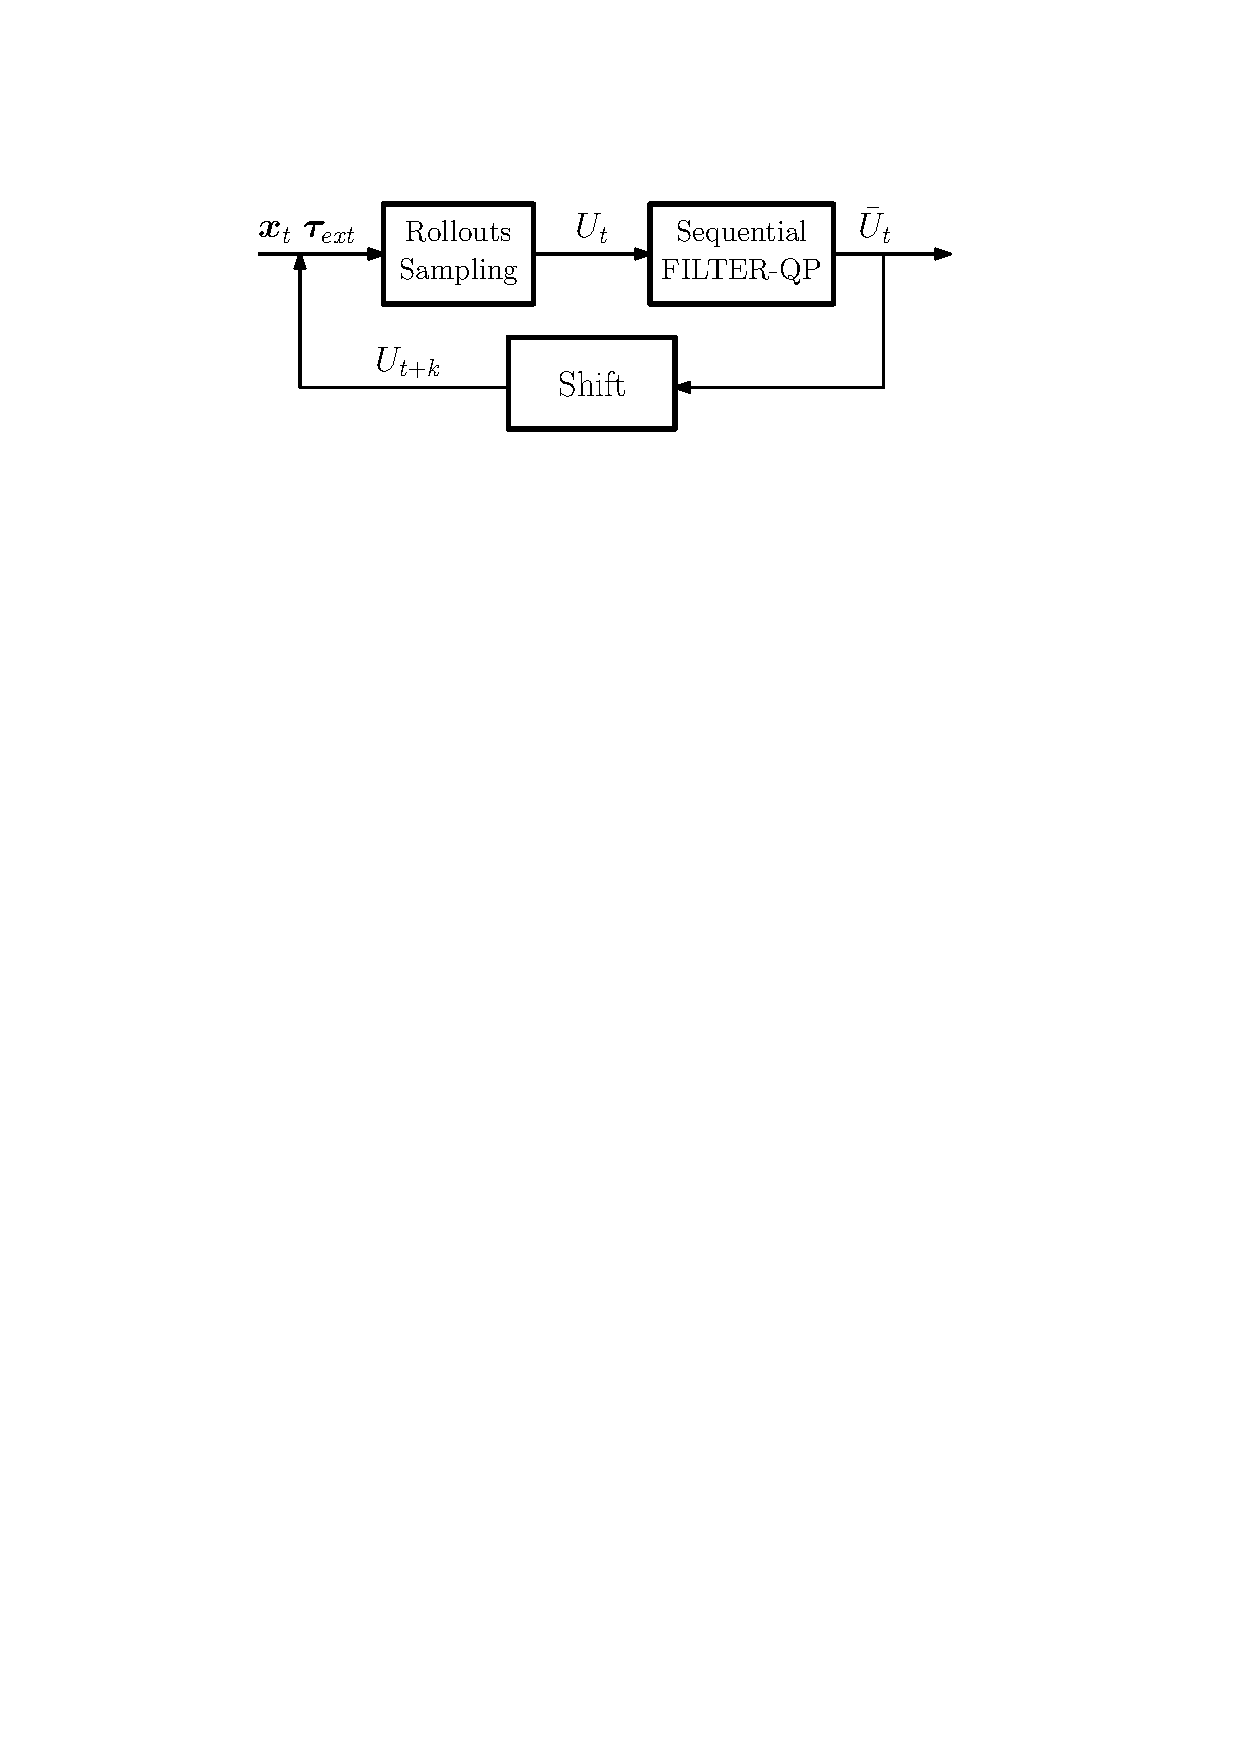
\includegraphics[width=0.8\columnwidth]{figures/schemes/stochastic_controller.pdf}
\caption{The sampling scheme is refined using the Sequential QP. The newly filtered trajectory is shifted in time and used to warm start the next sampling round.} \label{fig:sampling_scheme}
\end{figure}
